\chapter{Aufgabe 5}

Die Zentrale wird wie folgt geschützt (s. Abbildung~\ref{fig:firewall}):

\begin{itemize}
    \itemsep0.5em
    \item Der Webserver kommt in eine \textit{DMZ} und wird abgesichert durch einen Paketfilter $A$ durch den Zugriff von extern
    \item der interne Bereich der Zentrale wird wiederum durch einen Paketfilter $B$ abgesichert, der dafür sorgt, dass nur die HTTP-Requests durchgelassen werden, die für die Anwendungskommunikation notwendig sind.
    \item Der Datenbankserver ist im inneren Netz. Da wir in dem geg. Szenario davon ausgehen, dass der Webserver mit dem Datenbankserver kommuniziert, sichern wir den Datenbankserver durch einen weiteren Paketfilter ab.
    \item Der Webserver und der Datenbankserver sind zusätzlich durch Proxy-Server gesichert, damit ``gezielter auf Datenströme und vor allem deren Inhalte Einfluss`` genommen werden kann, zur ``Trennung und Inspektion der Kommunikation zwischen allen internen und externen Systemen`` (\cite[77]{ITS4}).
    Insbesondere die zusätzliche Abschirmung des Datenbankservers mit (womöglich) sensiblen (Kunden-)Daten schützt diese vor einer Kompromittierung des Webservers
    \item Zusätzliche Absicherungen der Server durch Antiviren-Software und regelmäßige Aktualisierung und einspielen von Patches durch die IT-Abteilung werden als selbstverständlich vorausgesetzt.
\end{itemize}

\noindent
Die Regeln für den (statischen) Paketfilter $A$ lauten vereinfacht wie folgt (wir gehen hierbei von einer \textit{Default Deny Strategie}\footnote{
s.~\cite[68]{ITS4}
} aus):

\begin{verbatim}
ACCEPT TCP FROM *,SSL_PORT TO WEBSERVER,443, SYN=1
ACCEPT TCP FROM WEBSERVER,443 TO *,SSL_PORT, SYN=0
\end{verbatim}

\noindent
Es wird hierdurch ein Verbindungsaufbau von Außen für die geg. Ports erlaubt.
Es sind nur Antworten in die andere Richtung möglich, der Webserver selber darf keine Verbindungen aufbauen (\texttt{SYN=0})\\

\noindent
Die Regeln für den (statischen) Paketfilter $B$ lauten vereinfacht wie folgt (wir gehen auch hier von einer \textit{Default Deny Strategie}):

\begin{verbatim}
ACCEPT TCP FROM WEBSERVER,* TO DATABASE,3306 SYN=1
ACCEPT TCP FROM DATABASE,3306 TO WEBSERVER,* SYN=0
\end{verbatim}


\begin{figure}
    \centering
    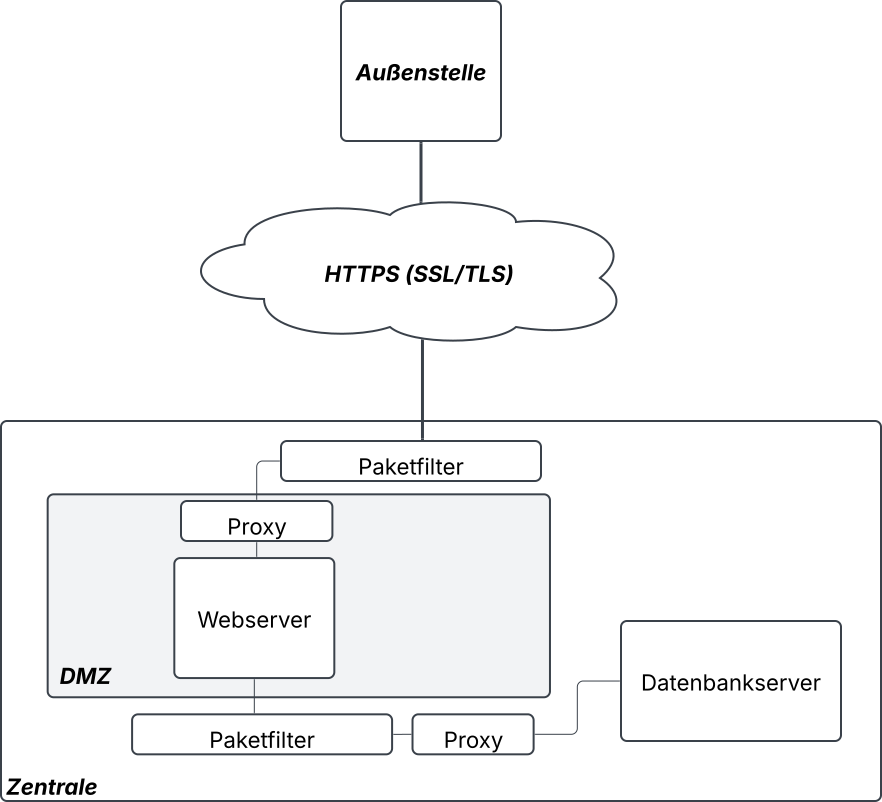
\includegraphics[scale=0.4]{aufgabe 5/img/firewall.svg}
    \caption{Vorschlag für eine Firewall-Lösung für das in Aufgabe 4 geg. Szenario (Quelle:eigene)}
    \label{fig:firewall}
\end{figure}
